%
% Modified by Megan Patnott
% Last Change: Jan 18, 2013
%
%%%%%%%%%%%%%%%%%%%%%%%%%%%%%%%%%%%%%%%%%%%%%%%%%%%%%%%%%%%%%%%%%%%%%%%%
%
% Modified by Bryce Frentz
% Last Change: 2018
%
%%%%%%%%%%%%%%%%%%%%%%%%%%%%%%%%%%%%%%%%%%%%%%%%%%%%%%%%%%%%%%%%%%%%%%%%
%
% Sample Notre Dame Thesis/Dissertation
% Using Donald Peterson's ndthesis classfile
%
% Written by Jeff Squyres and Don Peterson
%
% Provided by the Information Technology Committee of
%   the Graduate Student Union
%   http://www.gsu.nd.edu/
%
% Nothing in this document is serious except the format.  :-)
%
% If you have any suggestions, comments, questions, please send e-mail
% to: ndthesis@gsu.nd.edu
%
%%%%%%%%%%%%%%%%%%%%%%%%%%%%%%%%%%%%%%%%%%%%%%%%%%%%%%%%%%%%%%%%%%%%%%%%

%
% Chapter 2
%

\chapter{Experimental setup and procedures}
\label{chap: experiment}

\section{Introduction}

In this chapter, the details of the different experimental conditions for each phase of the dissertation are presented. Following that, sections are also included to highlight some techniques and equipment commonly used in low-energy nuclear physics, with an emphasis on those used in this work. The discussion is presented from the lens of the general to the specific, introducing general concepts for beam production and transport, acceleration systems, and radiation detection. Following the discussion of the scientific principles, even more detail about the facilities and equipment is given, highlighting differences between the facilities and techniques employed when compared to common equipment for nuclear physics experiments.



\section{Experimental Overview}
\label{sec: expOverview}


\subsection{Setup: cross section}
\label{sec: csMeasurement}

To measure the cross section of the $^{14}$N$\left( p,\gamma \right) ^{15}$O reaction, a campaign of experiments was performed at the University of Notre Dame Nuclear Science Laboratory (NSL) and at the CASPAR facility, part of the Sanford Underground Research Facility in Western South Dakota. More data about these facilities can be found in Sections \ref{sec: expND} and \ref{sec: caspar}, respectively. 

First, measurements were performed at the NSL in January 2018 to provide an above ground data set with which to compare to the underground measurements made at CASPAR throughout 2018. A schematic diagram of the setup used in these measurements is given in Fig. \ref{fig: setup} while pictures of the setup are shown as part of Fig. \ref{fig: casparPictures} and Fig. \ref{fig: actualSetup}. The schematic diagram, however, purposefully lacks the lead castle placed around the detector to shield from radiogenic background as it created a more confusing image. The effects of this lead shielding can be clearly seen in Fig. \ref{fig: backgroundComparison}. Additionally, these pictures are of the setup at the CASPAR facility, specifically. The equipment used and its placement was entirely the same for the data taken at either the NSL or CASPAR, less a few lead bricks. Therefore, these pictures are sufficient to present the setup for all phases of the experiment. 

At the NSL, the 5MV 5U single-ended Van de Graaf electrostatic accelerator was used to produce beams of $^{1}$H ions, created with the electron cyclotron resonance ion source, at energies ranging between 800 keV and 1200 keV. This energy range was chosen as it it provides an overlap to the CASPAR facilities capabilities and lower energies were prevented due to stability issues in the accelerator at the time. At the CASPAR facility, on the other hand, the $^{1}$H ions were created with a radiofrequency ion source and accelerated with a 1MV JN single-ended Van de Graaf electrostatic accelerator at energies ranging from 270 keV up to 1060 keV. This energy range is the entirety of the JN accelerator's operating range. While it is technically possible to push the accelerator down to voltages below 200 kV (and corresponding proton beam energies of $<$200 keV), doing so required a complete reconfiguration of the corona stack inside the accelerator and was deemed too insignificant a gain in measured data for the time that such a change necessitated. More detail on the operating principles of these accelerators and ion sources are given in Sections \ref{sec: accelerators} and \ref{sec: ion sources}, respectively. 

In both facets of the experiment, a magnetic dipole was used to select the desired beam after production. A combination of electrostatic and magnetic steering and focusing elements guided the beam to the target station through the beamline under vacuum. The principles upon which these systems operate are given in Section \ref{sec: beamline}.

The nitrogen targets for these experiments were both evaporated TiN and sputtered ZrN targets, all produced in Bochum, Germany. The TiN targets were backed with Ta while the ZrN targets were backed with W. All backings were machined to 2 inch squares before the addition of the active target material, after which point the corners were cut off so that the target would fit inside the holder. The targets were produced to nominal thicknesses of 50 nm (ZrN) and 100 nm (both ZrN and TiN). Targets were held in place during the experiment by securing them inside a target holder that was attached to the end of the beam line. To protect the targets from damage, the holder was connected to a water chiller which passed water through the back of the holder, cooling the targets constantly throughout the experiment. The use of rubber O-rings and hoses made the target holder electrically isolated from the rest of the beam line, allowing it to be used as a measure of the charge delivered directly, without the use of external Faraday cups. Additionally, to reduce carbon buildup on the target through the course of the runs, a cold trap was employed in front of the target for the measurements. This can be seen in Fig.\ \ref{fig: setup} and is detailed in Section \ref{sec: beamline}. The liquid nitrogen reservoir was filled every two hours, keeping the copper finger sufficiently cold throughout the duration of the measurements. 

In tuning, the beam spot on target was viewed with a quartz viewer or a MgO scintillation target, ensuring good quality of the delivered beam. In keeping the beam focues and centered through the runs, some of which lasted hours, pairs of upstream slits were utilized at both laboratories. These slits were moved to the edge of the beam at the end of the tuning process. When used together, a pair of slits defines a central line through which the beam passes to the center of the target. If the beam drifts or loses focus one (or more) of the slits will record a current. Thus, these enable a consistent delivery of beam to target throughout running. The locations of the slits, tuning elements, and the target stations at the NSL are presented in Figs.\ \ref{fig: nsl}, \ref{fig: staAnaSchematic}, and \ref{fig: targetRoom} while that information for the CASPAR facility is depicted in Fig.\ \ref{fig: casparSchematic}. Additionally, the beam delivered to the target at the NSL was in the range of 5 - 10 $\mu$A whereas at CASPAR it was on the order of 50 - 120 $\mu$A.

In this measurement, the $\gamma$-rays were observed with a coaxial p-type HPGe detector (manufactured by Canberra) rated with 130\% relative efficiency (relative to the efficiency of a 3" $\times$ 3" NaI detector with 1332 keV $\gamma$-rays). The HPGe detector was biased with +4000 V from an Ortec 660 Power Supply module. 1.5 mm of lead shielding was placed in front of the crystal's face to reduce the number of low-energy x-rays entering the detector ($<100$ keV photon energy) because they increase the dead time in the electronics decreasing processing time for signals of interest. A lead castle was built around the detector at each location to reduce radiogenic background from the target rooms. The arrangement of the lead around the detector was not the same between the two locations due to availability restrictions, but they provided similar background reduction at both locations.  The detector was placed at an angle of 55$\degree$ in order to minimize any angular distribution effects on the cross section, as that is the minimum of the second order Legendre polynomial which describes the angular behavior of the cross section. Additionally, the detector was placed on a sliding, isolating platform, enabling it's distance to the target to be easily changed. Measurements were primarily taken with the detector in close geometry, with only 2 mm between the target and the center of the lead shielding on the face of the detector (closer would have resulted in them touching on the corner because of their different orientation) but some were measured in far geometry, up to 25.4 cm between the target and lead shielding. This was done to provide a reference for the effects of summing on our detector response at high energies, which will be discussed further in Section \ref{sec: efficiency}. 

The electronics necessary for these measurements were minimal, since the HPGe detector has a pre-amplifier for signal processing attached to the charge recorder. Therefore, it was connected to an Ortec 672 Spectroscopic Amplifier with coarse gain set to 5, fine gain set to 10, Gaussian shaping, automatic pole zero adjustment, and a shaping time of 6 $\mu$s. Following this, the signals were sent to an Ortec 927 ASPEC Multichannel Analyzer (dual input model) which digitized the signals and was used in concert with the MAESTRO analysis software for recording the spectra. 



\subsection{Setup: lifetimes}
\label{sec: lifeMeasurement}


The goal of this measurement was to determine the lifetime of the 6.79 MeV state with a variety of target materials and nitrogen contents in order to identify any systematic effects which were unidentified in previous measurements (see Section \ref{sec: lifetimeLiterature}). In August 2019, this measurement was undertaken at the NSL using the Doppler Shift Attenuation Method (DSAM) in forward kinematics with the $^{14}$N$\left( p,\gamma \right) ^{15}$O reaction. Details of the DSAM can be found in Section \ref{sec: DSAM}. A schematic diagram of the setup used in these measurements, which was the same as used during the cross section experiments, is shown in Fig. \ref{fig: setup}. At the NSL, the 5MV 5U single-ended Van de Graaf electrostatic accelerator was used to produce beams of $^{1}$H ions, created with the electron cyclotron resonance ion source, at energies $E_{p}$ = 1020 keV and $E_{p}$ = 1570 keV, which provided good signal-to-background discrimination for the states of interest. At $E_{p}$ = 1570 keV, the $^{14}$N$\left( p,\gamma \right) ^{15}$O reaction also produced $^{15}$O nuclei in the 5.24 MeV and 6.18 MeV excited states, which have known lifetimes of $8.2 \pm 1.0$ fs and $< 2.5$ fs, respectively \cite{Ajzenberg-Selove1991}. Both of these states are also within the range of DSAM to measure, allowing additional verification of results for the measurement of the 6.79 MeV state in $^{15}$O.

After creation and acceleration of the $^{1}$H ion beam, a magnetic dipole selected the desired beam product and energy. A combination of electrostatic and magnetic steering and focusing elements guided the beam to the target station through the beamline under vacuum. The principles upon which these systems operate are given in Section \ref{sec: beamline}.

In tuning, the beam spot on target was viewed with a quartz viewer ensuring good quality of the delivered beam. In keeping the beam focues and centered through the runs, some of which lasted hours, pairs of upstream slits were utilized at both laboratories. These slits were moved to the edge of the beam at the end of the tuning process. When used together, a pair of slits defines a central line through which the beam passes to the center of the target. If the beam drifts or loses focus one (or more) of the slits will record a current. Thus, these enable a consistent delivery of beam to target throughout running. The locations of the slits, tuning elements, and the target stations at the NSL are presented in Figs.\ \ref{fig: nsl}, \ref{fig: staAnaSchematic}, and \ref{fig: targetRoom}. Additionally, the beam delivered to the target fell in the range of 20 - 50 $\mu$A.

For this experiment, implanted nitrogen targets were produced in July 2019 at the NSL and utilized for the measurement. Section \ref{sec: implantation} details the creation process and properties of the various fabricated targets. From these, the targets ultimately selected for use in the experiment were the high-dose Ta, W, and Mo implanted targets to highlight differences in backing materials while the low-dose Ta target was measured at the end of the experiment to provide a comparison on the nitrogen content in the targets. Specifically, these were selected to highlight the desired effects and be completed within the experimental time constraint. If more time had been available, all of the generated targets would have been studied for a complete mapping of the parameter space. The results of this undertaking as well as the data reduction and analysis necessary to arrive at those conclusions will be detailed in Chapter \ref{chap: lifetime}.

In this measurement, the $\gamma$-rays were observed with one of the GEORGINA detectors, a coaxial n-type HPGe detector rated with 100\% relative efficiency (relative to the efficiency of a 3" $\times$ 3" NaI detector with 1332 keV $\gamma$-rays). 1.5 mm of lead shielding was placed in front of the crystal's face to reduce the number of low-energy x-rays entering the detector ($<$100 keV photon energy) because they increase the dead time in the electronics. The detector was placed a rotating table with angular precision such that the detector's center could be placed within $\pm$0.5$\degree$ of the intended angle. Angles used in the course of the experiment were $0\degree$, $45\degree$, $60\degree$, $75\degree$, $90\degree$, $111\degree$, $135\degree$, and $-90\degree$. Measurements were taken with the detector in far geometry, with 25.4 cm between the target and lead shielding at the crystal's face. At this distance, the entire crystal face spanned an angular range of $\pm9\degree$. This measurement was also performed on the solid target beam line within the Sta. Ana target room, marked as the GEORGINA position in Fig. \ref{fig: targetRoom}. Unlike the cross-section measurement, however, the yield produced in the reaction is unimportant, so there was no need to account for efficiency or summing in this case. Additionally, to prevent any artificial peak shifting arising from gain shifts in the electronics to enter into the final product, the data were saved and the data acquisition restarted hourly at each angle. This allowed us to monitor for gain shifting throughout the experiment prevent it from obfuscating results. Ultimately, no evidence of gain shifting was found throughout the experiment. A CeBr detector was fixed at a backward angle of $-135\degree$ close geometry in order to provide a consistency check throughout the experiment.

The HPGe detector used for this measurement was biased to -4500 V with an Ortec 660 power supply module. It, like the detector used in the cross section measurements, comes with a pre-amplifier for signal processing. For this measurement, though, the Mesytech \textbf{ADC MODULE OF POWER} proved invaluable. It acted as the signal amplifier, analyzer, and digitizer. Through it, the settings applied were shaping time = 480, signal rise time = 40, pole-zero adjustment = 5000, gain = 1.24, and threshold = 320. This module comes with its own analysis software, \textbf{NAME OF SOFTWARE} for recording and saving the data files.



\section{Experimental Equipment}
\label{sec: equipment}



\subsection{Accelerators}
\label{sec: accelerators}

First and foremost, low-energy nuclear physics (generally understood to be the regime in which incident kinetic energies for reactions are below 1 GeV, often even as low as sub-MeV) requires particle acceleration systems in order to bring beams and targets together. The most common techniques for accelerating ions are 1) to use strong electrostatic fields for a straight-line acceleration, such as in the Van de Graaff accelerator, or 2)  by using a combination of electric and magnetic fields to accelerate the particles in cyclotron motion, aptly named a cyclotron. Van de Graaff accelerators are the most prominent of all accelerators, though, and are the type used in this work. 

The basic idea of a Van de Graaff accelerator is shown in Fig. \ref{fig: vdg principles}. The governing principle is that a beam of ions produced in an ion source (Section \ref{sec: ion sources}) are manipulated by additional electromagnetic elements (Section \ref{sec: beamline}) into an area of high electric potential. This high voltage is produced and maintained by continuously transporting positive charge from ground to a Faraday cage with a field free interior (referred to as the terminal, with voltage $V_{T}$). The positively charged ions, being in close proximity to the positively charged terminal feel a repulsive force, accelerating the ions out of the terminal and through the machine. Upon exiting the accelerator, the ions have energy

\begin{equation}
E_{ion} = qV_{T} = \dfrac{1}{2} m_{ion} v_{ion}^{2}
\label{eqn: accelerator}
\end{equation}

\noindent where $V_{T}$ again is the terminal voltage and $q$ is the charge state of the ion going through the accelerator, $m_{ion}$ is the mass of the ion, and $v_{ion}$ is the ion's velocity. When the terminal voltage is in MV, the beam energy is then provided in MeV. Specifically for the 5U accelerator, though, Equation \ref{eqn: accelerator} must be modified with an additional term. Inside the ion source, there is an electrostatic extractor, which transports the beam of ions out of the terminal and into the acceleration tube. With this correction, the beam energy for the 5U is given as

\begin{equation}
E_{ion} = q(V_{extractor} + V_{T}).
\label{eqn: beam energy}
\end{equation}

\begin{figure}
\centering
\includegraphics[width=0.5\linewidth]{figures/vdgDiagram.png}
\caption{A diagram of a Van de Graaff accelerator \cite{RolfsBook}. The charge transportation in this figure is shown with a belt, like the JN accelerator model at CASPAR, while the 5U accelerator at the NSL uses a Pelletron chain. }
\label{fig: vdg principles}
\end{figure}

The charge is delivered to the terminal via a mechanical delivery system. The 5U Sta. Ana accelerator at the NSL uses four Pelletron chains \cite{Herb1974}, each with its own power supply, while the JN Van de Graaff accelerator at CASPAR utilizes a rotating belt. In either case, the entire charging system is contained inside of a pressurized tank of insulating gas, SF$_{6}$ for the 5U and CO$_2$ for the JN, reducing the chance of a terminal discharge to ground from dielectric breakdown. This is not the only element to ensure the operational stability of the machine. The charging systems supply charge continuously to the terminal. However, charge is always being removed from the terminal via three primary pathways: 1) the beam of ions passing through the accelerator, 2) the resistive column, and 3) the corona system. In order to maintain stability, the currents that pass through these systems must always be in balance according to Kirchoff's Rule,

\begin{equation}
I_{chains} = I_{beam} + I_{column} + I_{corona}.
\end{equation}

\noindent The column is actually a series of equipotential hoops connected by equal resistors. Each conducting hoop provides a small step down in voltage from the terminal, ensuring that the beam of ions feel a smooth potential gradient throughout their acceleration. These can be seen in Fig. \ref{fig: column}, showing an interior view of Sta. Ana accelerator tank. 


\begin{figure}
\centering
\includegraphics[width=0.5\linewidth]{figures/inside5U.png}
\caption{View inside the Sta. Ana accelerator tank, showing the equipotential hoops as part of the column.}
\label{fig: column}
\end{figure}


The corona system is the real workhorse maintaining the stability of the accelerator's charging systems. As small irregularities can be present between different links in the Pelletron chains or the belt itself, the corona system is responsible for precise second-by-second compensation. The mechanical part of the system consists of an arm with sharp metal points on the end which can be moved towards and away from the terminal to draw away current. On the back end, however, it also is controlled by a voltage feedback system to adjust the current draw, keeping the terminal at a constant voltage. The feedback for the system is provided either by an external reference through a generating voltmeter or from the beam itself as it passes through an analyzing dipole magnet at the exit of the accelerator. As the beam passes through the magnet it will pass through a set of slits. If $V_{T}$ changes slightly, the energy of the beam will subsequently change, impacting the balance of the beam on the exit slits. This change in current will be fed back to the corona system, which in turn will compensate by changing the charge delivered to the terminal in order to maintain the slit balance. With this, $V_{T}$ can be kept incredibly steady, within roughly 1 kV for every MV on the terminal. This is the biggest advantage of a Van de Graaff accelerator over a cyclotron. Intrinsically, this acceleration system makes nuclear experiments possible through monoenergetic beams. 


\subsection{Ion sources}
\label{sec: ion sources}

A key item for the successful operation of any accelerator is the ion source, which produces the beams of charged particles used in experiments. Generating such beams is not a trivial task and, as such, many methods have been developed for achieving this. The two types relevant to this work, however, are the Electron-Cyclotron Resonance (ECR) ion source, used in the Sta. Ana accelerator at the NSL, and the radio frequency (RF) ion source, utilized in the JN accelerator at CASPAR.  Both systems are housed within their respective accelerator terminals, which acts as a Faraday cage and shields the internal components from external fields. Additionally, both systems operate on the same basic principle, namely that a given gas is ionized through the use of electron collisions in the source, but the mode of electron excitation is different. 

For the specifics of the ECR system, the 5U employs a Pantechnik Nanogen 14.5 GHz ECR source. This utilizes the cyclotron resonance of electrons (as the name obviously implies) to produce and maintain a plasma.


\begin{figure}
\centering
\includegraphics[width=0.5\linewidth]{figures/ecrSchematic.png}
\caption{Depiction of the interior of an ECR ion source with magnetic components labeled \cite{Melin1997}. This example shows a source operating from left to right, with the gas and RF generator inputs depicted as well as the exit for the ions. As discussed in the text, the combination of magnets confines the plasma in the center as it is pushed from left to right and out of the source.}
\label{fig: ecris}
\end{figure}


During operation, neutral gas (which includes the element to be accelerated as a component) is injected into a cavity surrounded by magnets. These magnets provide a superposition of axial and multipole fields in order to achieve a minimum at the center of the cavity increasing radially outwards with the goal of confining and stabilizing the generated ions. A cartoon depiction of such a system is presented in Fig. \ref{fig: ecris}. In order to generate the ions from neutral gas, a current is supplied to the chamber by a negative bias probe providing a constant supply of charge. From this, then, electrons are stripped and continually accelerated in cyclotron motion following the familiar cyclotron frequency relation:

\begin{equation}
\omega_{ecr} = \dfrac{e | B |_{ECR}}{m_{e}} = \omega_{rf}
\label{eqn: ecr}
\end{equation}

\noindent where $\omega_{ecr}$ is the frequency for the cyclotron resonance of electrons in a given magnetic field $B_{ECR}$, $e$ and $m_{e}$ are the charge and mass of the electron, respectively, and $\omega_{rf}$ is the frequency supplied by a radio radio-frequency (RF) power supply. This last term is included to highlight that during operation this is supplied externally and controlled in the use of the source in order to produce the plasma. After ionization, the magnetic configuration confines the plasma radially, while the axial magnetic field (provided by the extractor) pushes it through the cavity towards the exit of the source. Upon exiting the chamber and the Faraday cage of the terminal, the positive ions are next to a the positively charged terminal at high voltage, thus accelerating the ions. 

An ECR ion source has many advantages of over other common ion source designs. The primary advantage lies in its ability to deliver high-intensity beams (as much as hundreds of $\mu A$). For use in nuclear astrophysics experiments, such as the ones performed in this work, low cross sections are a problem to overcome, which is mitigated through this higher production. Additionally, due to the relatively simple restrictions on the inputs, these sources can provide a wide array of species, as they can produce beams of nearly anything that can be made into a gas, and exhibit long term stability, reliability, and longevity \cite{Melin1997}.  On the other hand, however, ECR ion sources also have some disadvantages compared to other common sources. One main drawback is that the ions are produced through the production of a plasma, meaning they are not directly controlled by any operational parameter \cite{Melin1997}. This leads to complicated tuning and sensitive operation, experimentally. Additionally, such sources are only capable of generating positive beams and can therefore only be utilized in single stage accelerators. Finally, due to the size of these ion sources and their necessary components, they are often impractical. In order to employ one in the Sta. Ana accelerator, the accelerator design had to be vertical. If the accelerator had been horizontal (like the other accelerators at the NSL) the torque generated by the ECR ion source would have shattered the acceleration column. Vertically, however, the source is stable inside the accelerator. Unfortunately, the choice to build and use the accelerator vertically is not one that every lab can make. 

The radio frequency (RF) ion source utilized at CASPAR operates on a very similar principle to the ECR ion source inside the Sta. Ana accelerator. A depiction of the RF ion source's components is given in Fig. \ref{fig: rfis}. In this case, the source chamber is a glass tube filled with a monoatomic gas, at CASPAR the only options are $\ce{^{1}H}$ and $\ce{^{4}He}$.  Electromagnetic coils are placed on both sides of this tube and generate RF waves in the tube, between the rings. In response to these waves, the electrons oscillate through and collide with the source gas, ionizing it. At the rear of the glass tube, an electrode supplies a constant, positive voltage (with respect to the terminal), forcing any ionized atoms towards the exit of the source. Upon leaving the source, as with the ECR ion source, the ions are accelerated because of their repulsion to the positively charged terminal. 

\begin{figure}
\includegraphics[width=\linewidth]{figures/rfSchematic.png}
\caption{Depiction of the interior of a RF ion source with magnetic components labeled \cite{Li2015}. The coils on either side provide the field to ionize the gas, whereas the probe on top provides the field necessary to extract the ions from the chamber.}
\label{fig: rfis}
\end{figure}

The RF ion source at CASPAR was also recently refurbished before installation, leaving it capable of beam production at even higher intensities than the ECR ion source inside the Sta. Ana accelerator. It can produce beams up to 150 $\mu A$, enabling similar high-intensity experiments. Another similarity to the ECR ion source is that it provides excellent operational stability and reliability. It does, however have significant drawbacks as well. The first and foremost of these is the degradation of the ion source canal. Operating the source causes a buildup on the exit canal of the source tube (higher intensity operation accelerates this process), necessitating significant maintenance. Additionally, the glass tube housing the plasma is quite sensitive. If power is supplied to the source when gas is not present, significant damage to the tube can occur. This is only mitigated with vigilant operation. The other major drawback is that the source is only capable of providing beams of two species (typically hydrogen and helium). In order to change the delivered species, a full tank opening and source alignment is required. 

Altogether, though, these sources are ideal for this work. They provide the necessary ion beams at high intensity, enabling the experiments. 




\subsection{Beam transport}
\label{sec: beamline}


Upon exiting the accelerator, the beam envelope contains a distribution of different masses, charges, and energies because the ion sources are indiscriminate in their production methods. For example, an ion source might produce some ionized diatomic gas, instead of monoatomic, like producing $\ce{^{1}H}+\ce{^{1}H}$ due to insufficient breakup of the source gas. However, all particles created in the same ionization state will have the same energy, dictated by Equation \ref{eqn: beam energy}. In order to filter such contaminants out of the beam, analyzing magnets are employed. These are typically 90$\degree$ dipole magnets, also utilizing the cyclotron motion of ions in a magnetic field in order to select a given type of particle at a specific energy. These magnets are typically located at the exit of accelerators, and, due to their fixed size, have a fixed radius, $R_{am}$, through which a beam can pass. Therefore, for a given particle of mass $m$, energy $E$, and charge state $q$, the magnetic field, $B_{am}$, inside the analyzing magnet can be tuned to allow through only a specific particle/energy combination by

\begin{equation}
B_{am} = \dfrac{\sqrt{2 m E}}{q R_{am}} = \dfrac{\sqrt{2m}}{q R_{am}} \sqrt{E} = k \sqrt{E}
\label{eqn: analyzingMagnet}
\end{equation}

\noindent, where $k$ is a constant for a unique combination of particle and charge state. This separates the in-beam contaminants from the ions of experimental interest.  

In order to deliver the beam of ions to the target chamber and experimental hall, a series of steering and focusing elements are placed along the beam pipes. As the beam is self-repulsive due to it all being the same charge, these are necessary to contain the beam and keep its intensity at acceptable levels for experimental purposes. They also allow adjustment of the beam's position in order to deliver it to a specific experimental setup and allowing for simple transitions between different target locations. A schematic of the Sta. Ana and its beam transportation equipment is provided in Fig. \ref{fig: staAnaSchematic}. 


\begin{figure}
\centering
\includegraphics[width=0.7\linewidth]{figures/staAnaSchematic.png}
\caption{Schematic of the Sta. Ana accelerator at the NSL and its associated beam line. The target room containing experimental equipment is located after the switching magnet and is highlighted later (see Section \ref{sec: expND}). For the implanted target production (see Section \ref{sec: implantation}) occurred at the implantation station off the neutron dipole, shown in this figure.}
\label{fig: staAnaSchematic}
\end{figure}

Vacuum systems are important components of the beam production and experimental operation. All experimental components, like the ion source chamber, acceleration tubes, target chamber, and connecting beam pipes need to be free of residual gas. If not, the beam quality would suffer dramatically, collisions of the beam with the remaining atmosphere would cause significant intensity and energy losses, preventing transport and, ultimately, the measurement. In order to maintain an experimental vacuum level (typically $\sim 10^{-7}$ Torr), a series of metal pipes run from the ion source to the target chamber. These are connected by air-tight gaskets and have isolating valves employed with high-vacuum pumps (cryogenic or turbomolecular) along the line. These enable easier maintenance or changing of experimental conditions without destroying the vacuum created through the entire beam line. Without high-vacuum, there would be additional adverse effects on the target quality. Contaminants, typically hydrocarbons, present in residual gas can accumulate on the surface of the target due to the beam heating the surface. This is unwanted, as it not only provides an additional layer of energy loss for the beam before interacting with the target but also a significant contaminant in experimental results due to carbon's high cross-section.

Besides maintaining clean, high-vacuum near a target, another common method for reducing the carbon build-up on experimental surfaces is to utilize a so called cold trap in front of a target. A cold trap is is a liquid nitrogen cooled copper pipe designed to be nearly the same size and shape as the beam pipe to prevent it from interfering with an experiment. An example of a cold trap like the one used in this work is shown in Fig. \ref{fig: setup}. The cold trap works much like a cryogenic pump. By cooling the copper pipe with liquid nitrogen, the residual hydrocarbons in the beam pipe and target chamber will condense on the surface of the pipe, trapping them before most can reach the target and cause carbon buildup. A common practice, which we also employed in this work, is to apply a negative voltage to the cold trap, forcing electrons scattered by the collision of the beam with the target back to the end of the chamber and providing an accurate reading of the amount of beam delivered to the target. 


\begin{figure}
\centering
\includegraphics[width=0.8\linewidth]{figures/expSetup.png}
\caption{Depiction of the experimental setup used in this work, including the angled target holder, HPGe detector, and cold trap.}
\label{fig: setup}
\end{figure}



\subsection{Radiation detection}
\label{sec: detectors}

Generally speaking, the first step in the design of an experiment is understanding the necessary detection system to match the reaction. This is because, like a child trying to reconstruct a broken Lego set, measurements are done by measuring the products of a reaction and trying to work backwards to understand its form and function. In nuclear physics experiments, there are three primary classes of radiation to consider as the reaction products: 1) energetic charged particles, 2) neutrons, and 3) electromagnetic radiation (photons). Of these, the first class can be further subdivided into heavy ions, like the proton, $\alpha$ particle, or other nuclei, versus light particles, namely electrons. For all classifications of particles, they are detected primarily through energy deposition into another medium, with the specific interaction dependent on the type of particle. These methods will be introduced below, but the reader is referred to \cite{KnollBook} for a complete discussion of radiation interaction with matter and subsequent detection techniques.  

For example, for charged particles in class 1, the dominant mechanism for energy deposition is through collisions with atomic electrons mediated by the electromagnetic force. As the particles pass through a medium, it generates an electromagnetic field in the surrounding space, which induces excitation in atomic electrons and even ionization if the energy is large enough. Each such interaction results in energy transfer from the incident particle to its neighborhood, slowing it to an eventual stop (usually). In many cases, the particle will stop inside the material, meaning that all of the energy was deposited. On the other hand, it is possible for the particle to pass outside of the medium due to its trajectory, meaning that only a fraction of the total energy from the particle will be deposited in the material. The path a particle traces through a medium is dependent primarily on its own properties, like mass, as heavier particles are more resistant to changes in momentum from interactions with atomic electrons, while an electron's path in a medium is typically chaotic, with significant scattering from interactions with other electrons. The detection medium thus plays little part in the detection of charged radiation.

Neutrons, by contrast, interact significantly differently with matter because of their electrically neutral state. Because they cannot react via the electromagnetic interaction, they can only exchange energy with their surrounding through the strong nuclear interaction. This implies that they will only have meaningful interactions with atomic nuclei inside of the detection material. This presents a significant challenge, however, as atomic nuclei occupy only a minuscule volume of space. This makes the medium in which the neutrons are detected much more important. In order to increase the probability of detection, the medium would ideally have a higher density, increasing the number of potential interaction sites for the neutron. Unfortunately, this can introduce another problem, as higher density materials are often those with higher mass nuclei as constituents. While such material will have a greater chance to interact with the incident neutrons, these heavy nuclei will not acquire significant energy in collisions due to conservation of energy and momentum, similar to how the momentum of heavy charged particles is largely unaffected by interactions with atomic electrons. As such, a neutron traveling in a high-density material with heavy nuclei may bounce chaotically many times before exiting the medium without depositing enough energy to produce a strong enough signal to be detected by the system's electronics. Therefore, in the detection of neutrons, the medium is almost always chosen to be composed of light elements, which are more favorable for the detection of neutrons as each collision will produce a more significant exchange of energy with the medium. Materials with a high neutron cross section, like boron on $\ce{^{3}He}$, are typically chosen as detection media. Due to the challenges of detecting high-energy (several MeV or greater) neutrons, a common technique for experiments involving neutrons is time-of-flight. In these cases, it is extremely unlikely to capture all of the neutron energy in a detection medium, so by measuring the time between neutron emission and interaction in a detector at a known distance the velocity, and kinetic energy, of the neutron is determined. This, however, necessitates a detailed understanding of the timing characteristics of a detector medium.

Finally, for quanta of electromagnetic radiation, or photons the interaction proceeds through yet different means. As an electrically neutral particle, photons do not interact with the medium in general and only at discrete points through the atomic electrons. As such, the interactions are much more probable than those of the neutron while being less than those of charged particles. Similar to charged particles, though, it is highly likely that photon interactions with matter result in a much higher chance to deposit all of the photon's energy in the medium. Clearly, by increasing the elemental number of the detection material's constituents, the probability of interaction with photons increases by increasing the number of possible interaction sites. As such, higher $Z$ materials are preferred for the detection of photons. 

On balance, there are three primary modes for photons to interact with matter: 1) the photoelectric effect, 2) Compton scattering, and 3) electron-positron pair production \cite{KnollBook}. Fig. \ref{fig: radiationInteraction} illustrates these possible interactions and Fig. \ref{fig: gammaSpec} depicts the ways in which these effects manifest in measured spectra. 


\begin{figure}
\centering
\includegraphics[width=0.8\linewidth]{figures/photonInteraction.png}
\caption{Depiction of the modes for photons to interact with matter, showing a) the photoelectric effect, b) Compton scattering, and c) electron-positron pair production. }
\label{fig: radiationInteraction}
\end{figure}


In photoelectric absorption, the photon transfers its energy to an atomic electron, leaving it in an excited state or ionizing it completely, where the electron deposits its energy like any other charged particle. If ejected, the electron will have energy $E_{e}$:

\begin{equation}
E_{e} = E_{\gamma} - E_{b}
\end{equation} 

\noindent where $E_{\gamma}$ is the incident photon energy and $E_{b}$ is the binding energy of the electron. In these cases, the electron is most likely ejected from the innermost atomic shell. For low-energy photons (below $\sim$1 MeV), this is the dominant interaction process \cite{KnollBook}. 

Compton scattering is a similar process in that it also ends up producing an energetic electron inside the detection medium. In this type of interaction, a photon scatters inelastically from an atomic electron, imparting some of its energy to the electron and changing the momentum of both. Unlike the photoelectric effect, not all of the photon's energy is absorbed by the electron. As such, any of the interactions can occur again in the medium, like subsequent scatterings, full photoelectric absorption, or pair production, or the scattered photon could leave the material entirely. For the former conditions, the full energy of the photon will still (likely) be absorbed in the material. However, in the event that a subsequent scattered photon leaves a detection medium, this will manifest in the total energy measured in this event being lower than the true incident photon energy, artificially reducing the true signal and increasing the background. This is known as the Compton edge, which is shown in Fig \ref{fig: gammaSpec}. This effect is also the dominant effect in cases where the phtoon has a middle range of energies (between $\sim$ 1 - 6 MeV) \cite{KnollBook}.

The final mechanism by which photons interact with matter is through electron-positron pair production, often shortened to just pair production. This occurs when a photon traveling spontaneously transforms into a matter-antimatter pair, the electron and positron, respectively.  This effect is induced by an interaction with a virtual photon from the electromagnetic field in the space the real photon is traveling. For this to occur, the photon's energy must be greater than the rest mass-energy of the pair, namely 1.022 MeV for electron-positron. After creation, the pair will share the total original energy (less their rest mass-energy) and momentum of the photon in their subsequent kinetic energies and momenta. From this point, the electron will continue to scatter and deposit energy in the normal manner for charged particles, while the positron will annihilate with one of the atomic electrons in the surrounding material, creating to diametrically opposed gamma-rays at 511 keV. With these, there are three potential outcomes: 1) the two new photons will interact with the surrounding medium through the processes already detailed, depositing their energy, and resulting in the total deposition of the initial photon's energy in the detection medium; 2) one of the new 511 keV photons will leave the detector without interacting and result in a deposition of the total initial energy less 511 keV; 3) both of the subsequent 511 keV photons leave the detector, resulting in an energy deposition of the total initial photon's energy minus 1.022 MeV. The two situations where a subsequent photon leaves the material are more comon with higher initial photon energies, manifesting in their own peaks in a measured spectrum. These are called escape peaks, shown in Fig. \ref{fig: gammaSpec}, with the single escape peak being when one photon leaves the medium and the double arising when both 511 keV photons escape the system. Whereas the full deposition of the photons energy is also shown in that spectrun and known as the full-energy peak. 

\begin{figure}
\includegraphics[width=\linewidth]{figures/photonSpectrum.png}
\caption{Cartoon depiction of an example experimental spectrum for photon interactions \cite{Hall2018}. Artifacts from the ways in which photons interact with matter are highlighted in the spectrum and are common in experimental gamma spectra.   }
\label{fig: gammaSpec}
\end{figure}


This work is concerned ultimately with measuring photons as reaction products and employed high-purity germanium (HPGe) semiconducting detectors for that purpose. These are characterized by having a relatively small band gap between the electrons within the valence and conducting bands. When photons enter the Ge crystal, they excite electrons across the band gap from the valence to the conducting band, leaving behind vacancies, known as holes, in the valence band. These excited electron-hole pairs feel an electric field supplied by the detector's bias voltage, causing them to drift to the charge collection electrodes at the end of the crystal, resulting in an electric current pulse. Since HPGe has a small band gap, around 0.7 eV (depending on impurities) \cite{KnollBook}, it requires constant cooling of the medium by liquid nitrogen in order to reduce the number of electron-hole pairs created by thermal excitations in the valence band. However, by cooling these detectors, HPGe becomes extremely useful because of the large number of charge carries produced by the small band gap in an energy deposition event, giving superior energy resolution. It is for this reason that HPGe detectors are ubiquitous in nuclear physics laboratories around the world - even those shown in movies. Comparatively though, HPGe detectors are more expensive and (typically) less efficient than NaI detectors, which are the other primary type of photon detector, so they are not which downsides to use as well. 

Thus, in every experiment it is important to anticipate reaction outcomes when planning what type of radiation detection system to employ. As stated, this work was concerned with the measurement of high-energy photons from a nuclear reaction, so we chose to use HPGe detectors for their superior resolution.




\section{Cross-section measurements}
\label{sec: cs experiment}

This set of data was taken over the course of five separate experiments. The first occurred at the University of Notre Dame's Nuclear Science Laboratory (NSL) in January of 2018 and covered the proton energy range of E$_{p}$ = 800 - 1200 keV. The experiment was then continued at the Compact Accelerator System for Performing Nuclear Astrophysics (CASPAR) facility at the Sanford Underground Research Facility located in Lead, South Dakota in three increments: February 2018, May 2018, and August / September 2018. These measurements covered the energy range from E$_{p}$ = 270 - 1100 keV, in order to measure the $^{14}$N$\left( p,\gamma \right) ^{15}$O reaction cross-section to compare the performance of the CASPAR facility to an above-ground laboratory.


\subsection{Experiment at Notre Dame}
\label{sec: expND}

The goal of this experiment was to measure the $^{14}$N$\left( p,\gamma \right) ^{15}$O reaction cross-section in a low energy range of the Sta. Ana accelerator, proton energy range of E$_{p}$ = 800 - 1200 keV, to provide a self consistent data set with which to compare the results of a measurement at CASPAR. Owing to the difficult experimental environment at CASPAR, this also allowed a dry-run of the procedures and an opportunity to work out kinks with the equipment before moving underground. The Notre Dame Nuclear Science Laboratory's (NSL) layout is shown in Fig. \ref{fig: nsl}, with this phase of the measurement occurring on the Solid Target beam line, a schematic of which is shown in Fig. \ref{fig: targetRoom}. A diagram of the specific setup used in this experimental phase is depicted in Fig. \ref{fig: setup}. In order to reduce confounding effects, it was also employed identically at CASPAR. 


\begin{figure}
\includegraphics[width=\linewidth]{figures/nslLab.png}
\caption{The Notre Dame Nuclear Science Laboratory, with experimental areas important for this work identified. }
\label{fig: nsl}
\end{figure}

\begin{figure}
\includegraphics[width=\linewidth]{figures/targetRoom.pdf}
\caption{Schematic of the Sta. Ana accelerator's target room, showing all experimental stations. The solid target beam line used in this experiment is emphasized for clarity. For these experiments, the target chamber and detectors were placed at the location named Georgina. } 
\label{fig: targetRoom}
\end{figure}





\subsection{The CASPAR facility}
\label{sec: caspar}

In an attempt to extend the data range down to the lowest possible energies and provide a proof-of-principle for the facility, a second phase of the experiment was performed at the CASPAR facility. CASPAR is the Compact Accelerator System for Performing Astrophysical Research, located on the 4850 ft level of the Sanford Underground Research Facility, and is the first underground accelerator facility in the United States. This facility was originially the Homestake Gold Mine in Western South Dakota, just outside (and underneath) the town of Lead. It is also the location of the famous Ray Davis and John Bahcall underground neutrino experiment in which the solar neutrino problem was identified \cite{Bahcall1976}. The accelerator located at the facility is the recently refurbished JN Van de Graaff, which had been employed at the NSL since its arrival in the early 2000's. Fig. \ref{fig: casparPictures} shows some pictures of the facility while Fig. \ref{fig: casparSchematic} provides a detailed schematic of the equipment available at the CASPAR facility. 


\begin{figure}
\centering
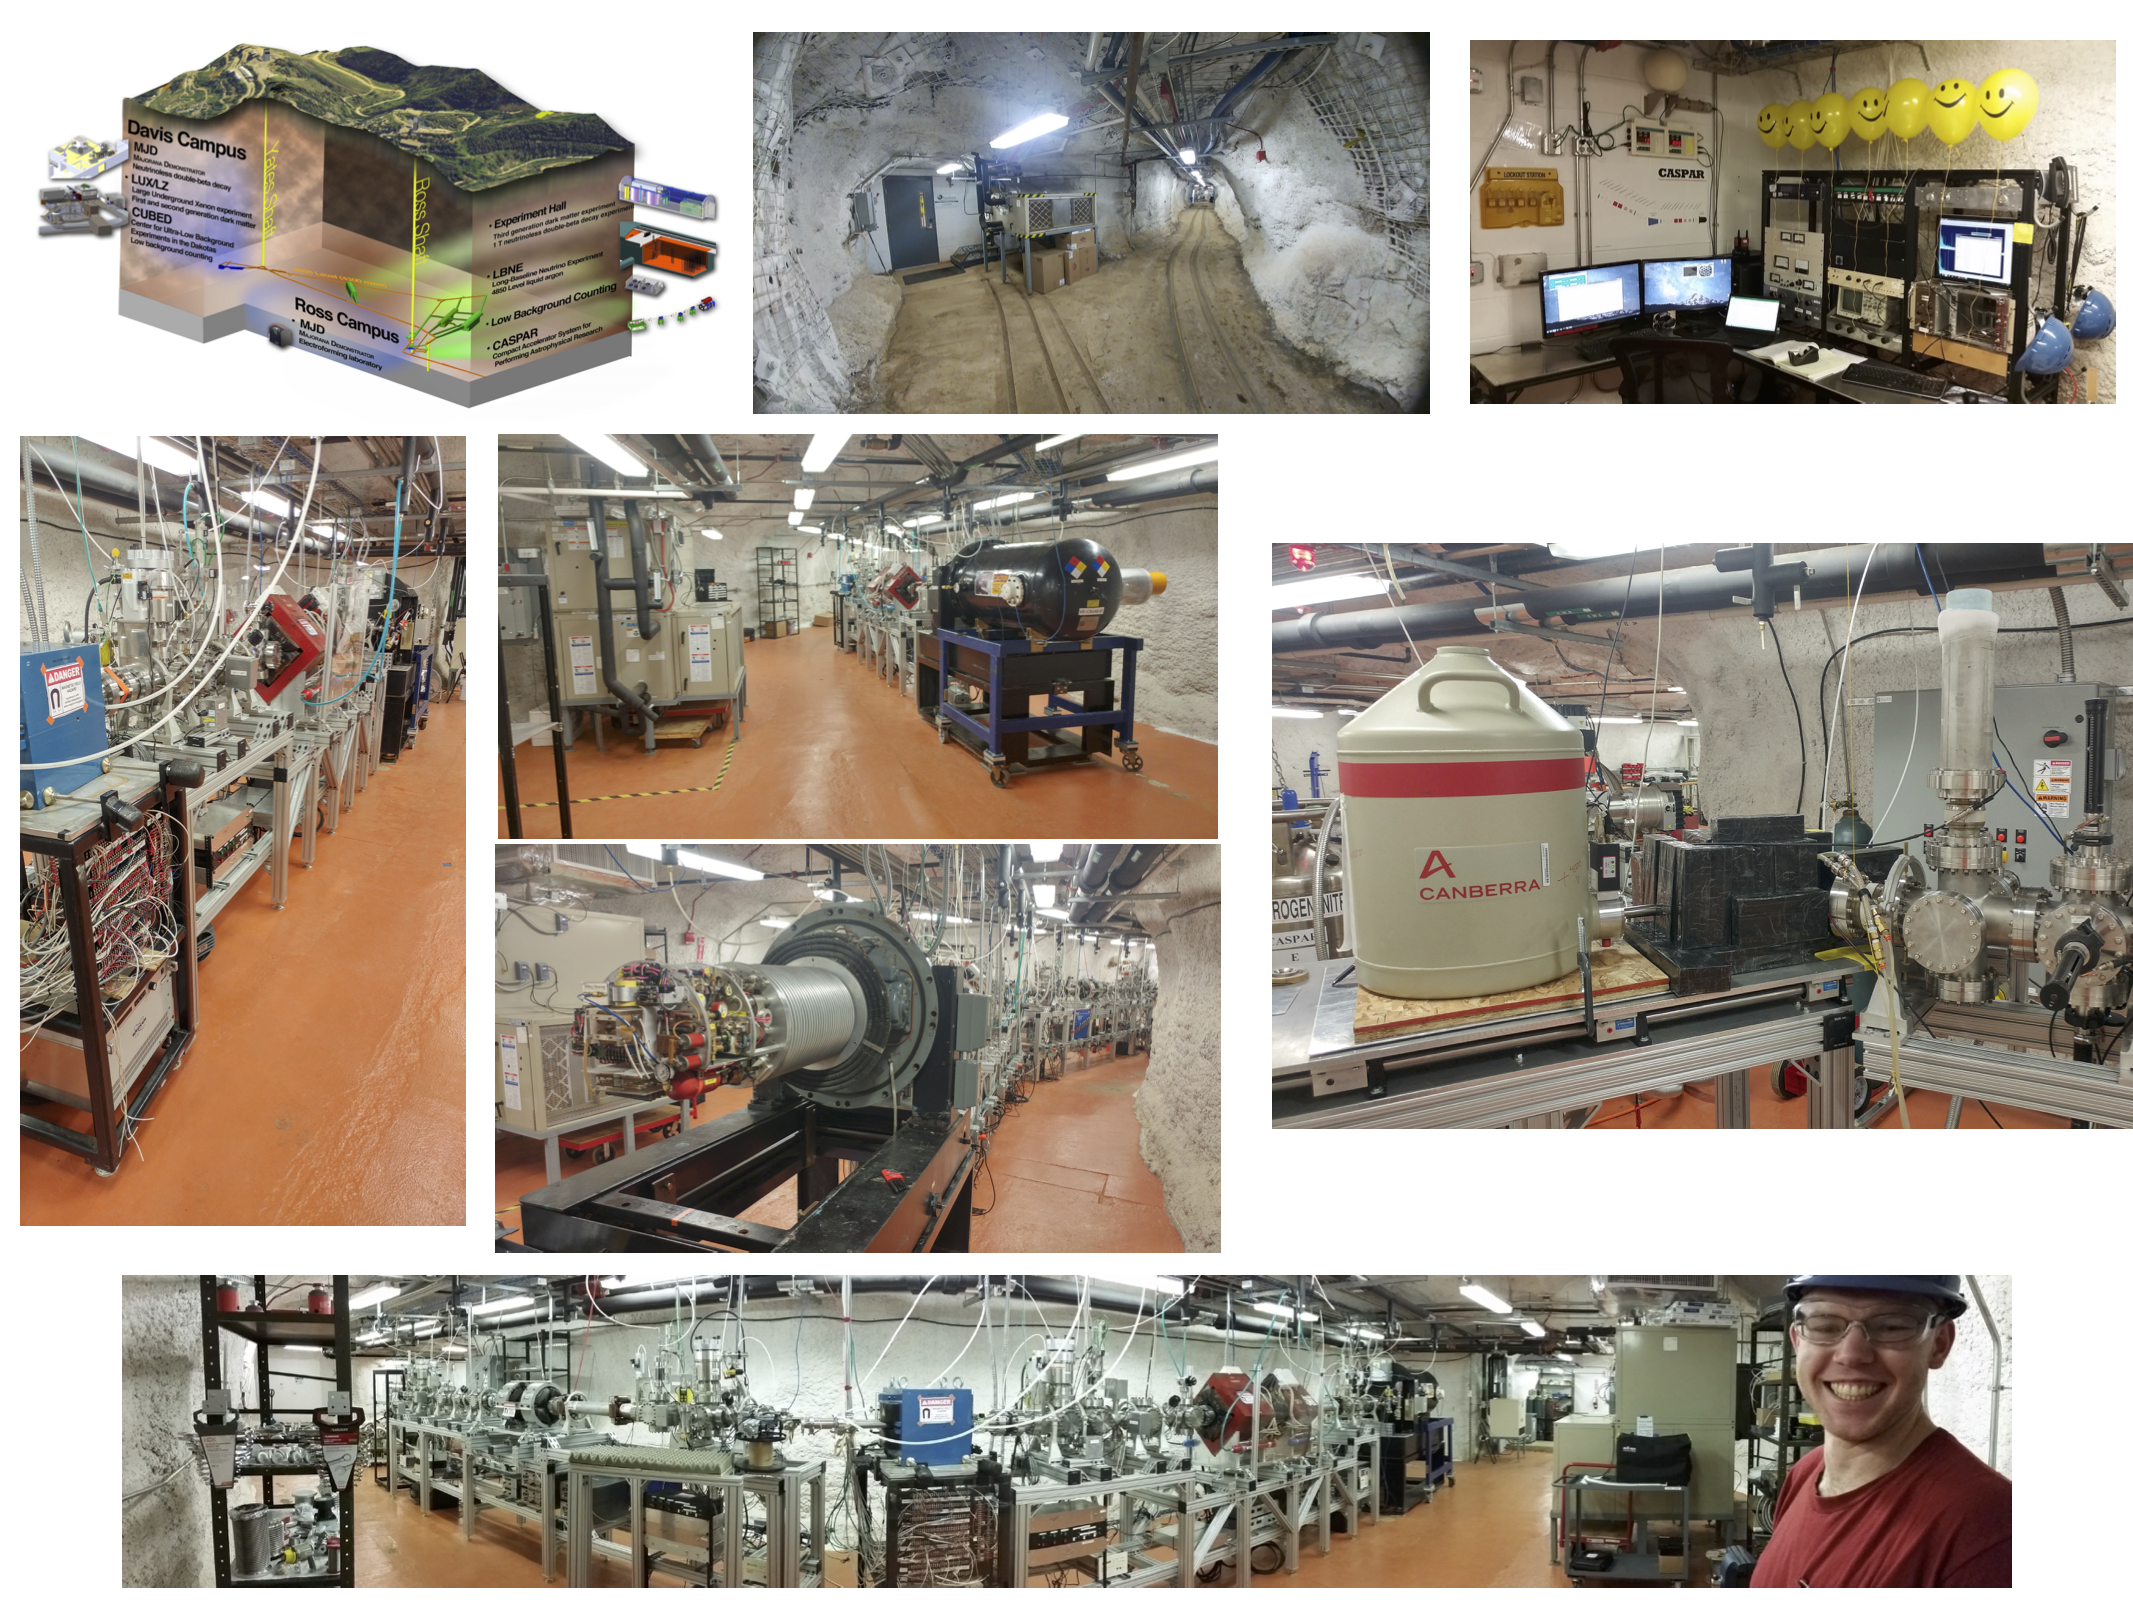
\includegraphics[width=\linewidth]{figures/casparPictures.png}
\caption{Pictures of the CASPAR facility. }
\label{fig: casparPictures}
\end{figure}



\begin{figure}
\centering
\includegraphics[width=\linewidth]{figures/casparSchematic.pdf}
\caption{Schematic of the equipment employed at the CASPAR facility. In this case, the figure is read right-to-left, with beam generated in the JN accelerator on the right of the figure. }
\label{fig: casparSchematic}
\end{figure}



Some of the problems with performing low-energy nuclear astrophysics measurements were detailed in Section \ref{sec: thermonuclear reaction rates}. The most significant of these is the diminishing cross section at astrophysically relevant energies due to Coulomb repulsion. There are a number of techniques for mitigating this problem: 1) extrapolating from higher energy with techniques like $R$-matrix (see Section \ref{sec: r-matrix}), 2) increasing the reaction yield with high-intensity accelerators and targets, 3) performing long term measurements to enable measurements of ridiculously low cross section reactions, and 4) drastically reduce cosmic background to increase the signal to background ratio and prevent these events from hiding a signal of interest. Of these, CASPAR is equipped to employ the solutions of 2, 3, and 4. In Section \ref{sec: ion sources}, the RF ion source utilized inside the JN accelerator was described, but the useful feature is that it can deliver proton and $\alpha$ beams up to 150 $\mu A$, increasing the experimental yield dramatically. Additionally, without the constraints and competition of multiple running groups, which is the reality at larger labs like the NSL or the National Superconducting Cyclotron Laboratory at Michigan State University, the facility is able to measure a reaction as long as necessary (five weeks in this case). Finally, with nearly a mile of rock cover above the facility provided by the mountains, the facility has excellent passive shielding. The background reduction compared to a surface laboratory like the NSL is shown in Fig. \ref{fig: backgroundComparison}. Strictly speaking, due to the high content of the uranium and thorium decay chains in the surrounding rock, the radiogenic background (that at energies below $\sim$2.6 MeV) is actually higher at the CASPAR facility than the surface. This, however, can be (and is) addressed by adding additional lead shielding around the detector crystal. Taken together, these features advance CASPAR beyond the capabilities of other laboratories performing nuclear astrophysics experiments and make it particularly useful. It's for these reasons that it was chosen to perform the low-energy phase of this work. 


\begin{figure}
\centering
\includegraphics[width=\linewidth]{figures/casparBackgrounds.png}
\caption{Background $\gamma$ spectrum taken at the NSL, CASPAR, and CASPAR utilizing passive lead shielding, with a) showing the full spectrum and b) showing a subset of the spectrum at low energies to highlight the radiogenic background, which is higher at CASPAR without lead shielding. Clearly, the facility provides a prodigious reduction of cosmogenic background, making the facility advantageous for low-energy nuclear astrophysics experiments.}
\label{fig: backgroundComparison}
\end{figure}



Additionally, the JN accelerator at CASPAR expands on the potential measurement range compared to the LUNA II facility, the other preeminent underground nuclear astrophysics laboratory in the world \cite{Formicola2003a}. The two have similar background reduction due to their environments and equal capacity to perform extensive measurements. However, until the LUNA-MV facility is completed \cite{Broggini2010, Ferraro2018}, CASPAR's expanded energy regime makes it the only facility with the capability to overlap with those measurements performed at surface laboratories, making it the ideal facility for low-energy nuclear astrophysics. 

The measurements at CASPAR were undertaken over the course of five weeks in February 2018, May 2018, and August / September 2018. These covered the proton energy range from E$_{p}$ = 270 - 1060 keV, overlapping with the measurements at the NSL. As stated in Section \ref{sec: expND}, the equipment like detector, electronics, and overall setup used in this campaign was the same as what was used at the NSL. The only significant different was the different targets used in this experiment. These were sputtered ZrN targets of varying thickness (50 - 100 nm sputtered layer thickness, 11 - 22 keV thick for protons at 278 keV) produced specifically for this experiment in Bochum, Germany. The targets were produced by sputtering a layer of Zr onto a W backing in a nitrogen atmosphere. Given the high intensity of the beam delivered at CASPAR, these were constantly monitored for degradation and carbon buildup to reduce target effects on the measurement. 





\section{Lifetime measurement}
\label{sec: lifetime experiment}

The goal of this measurement was to determine the lifetime of the 6.79 MeV state in $^{15}$O with a variety of target materials and nitrogen contents in order to identify any systematic effects which were unidentified in previous measurements. Targets for this measurement were produced at the NSL in the summer of 2019. The process of fabricating these targets is presented in Section \ref{sec: implantation}. When measuring the lifetime, the $^{15}$O nuclei were generated using the  $^{14}$N$\left( p,\gamma \right) ^{15}$O reaction at energies ranging from 1020 keV to 1540 keV. At these energies, the excited states in $^{15}$O at 5.24 MeV and 6.18 MeV, with known lifetime, are also populated. The details of how these measurements were made are given in Section \ref{sec: lifetimeND} By measuring all of these, these additional states can be used as a check to ensure the validity of the measurement technique used herein: the Doppler Shift Attenuation Method. 


\subsection{The Doppler-Shift Attsenuation Method for lifetime measurements}
\label{sec: DSAM}


Nuclear lifetimes are important observables to measure because they provide a link to understanding the strong nuclear force. They are necessary to determine the reduced transition probabilities which are one of the most important probes of nuclear structure and the forces governing the behavior of nuclei.The Doppler Shift Attenuation Method (DSAM) is a well characterized method for determining the lifetimes of excited nuclear states that decay via gamma emission in the range of 10$^{-11}$ - 10$^{-15}$ s \cite{Blaugrund1966}. The ranges where DSAM is applicable are compared with other common methods for determining nuclear lifetimes in Fig. \ref{fig: lifetimeRanges}. 


\begin{figure}
\includegraphics[width=\linewidth]{figures/lifetimeTechniques.png}
\caption{Ranges over which the different lifetime measuring techniques are valid (Obtained via personal communication with M.K. Smith in 2017).}
\label{fig: lifetimeRanges}
\end{figure}


The basic idea of DSAM is to produce an excited nucleus inside of a dense target in which the reaction product will decay. The de-excitation of the nucleus then takes place either while the nucleus is slowing down or after it stops, depending on the lifetime of the specific state and the stopping within the target. Then, as is true with the classical Doppler shift, the energy of the emitted $\gamma$-rays are shifted depending on their emission angle relative to the motion of their source, the decaying nucleus. Thus, $\gamma$'s emitted at different velocities during the slow-down and detected at given angles will have a spread of energies. Specifically, for a given nucleus decaying at a time $t$ with a speed of $v(t)$, the Doppler shifted energy of the gamma ray, $E_{\gamma}$, is 

\begin{equation}
E_{\gamma} = E_{0} \left(1 + \dfrac{v(t)}{c} \cos (\theta)   \right),
\label{eqn: doppler1}
\end{equation}

\noindent where $E_{0}$ is the energy of the decay for a nucleus at rest, $c$ is the speed of light, and $\theta$ is the lab angle between the momentum vectors of the decaying nucleus and gamma ray, respectively. A depiction of this scenario is given in Fig. \ref{fig: decay}.

\begin{figure}
\includegraphics[width=\linewidth]{figures/decay.pdf}
\caption{A generic nuclear reaction showing the creation of an excited nucleus and subsequent decay, causing a Doppler shift in the measured energy of the $\gamma$ ray.}
\label{fig: decay}
\end{figure}


As the nuclear decay process is statistical in nature, the measured spectrum of gamma energies for a particular transition is a continuous distribution of energies from the unshifted, rest energy peak to the maximally Doppler shifted peak. As Equation \ref{eqn: doppler1} was specific to a single transition, it is necessary to consider the entire sample of decays measured. By defining the average velocity of all nuclei at the time of decay, $\overline{v}$, the initial velocity of all recoiling nuclei, $v_{0}$, and their ratio, $F(\tau)$, called the attenuation factor, it is possible to relate the behavior of the entire distribution to the lifetime of the state. This is 

\begin{equation}
E_{\gamma} = E_{0} \left(1 + F(\tau) \beta_{0} \cos (\theta)   \right),
\label{eqn: dopplerFull}
\end{equation}

\noindent where $\beta_{0} = v_{0}/c$ is the relativistic velocity factor. $F(\tau)$ therefore provides an analytical relation between the nuclear lifetime and the measured Doppler shift, given by Blaugrund in 1966 \cite{Blaugrund1966} as

\begin{equation}
F(\tau) \beta_{0} = \dfrac{1}{\tau} \int_{0}^{\infty} \beta(t) \exp \left( \dfrac{t}{\tau} \right) dt,
\end{equation} 

\noindent where $\beta(t) = v(t)/c$ is the time dependent relativistic velocity factor. The devil, however, is in the details of calculating $\beta(t)$, since it is reliant on stopping powers of the nuclei in the target material, implying an accurate knowledge of the target composition and population pattern of the nucleus. In some cases the feeding is not well known and for nearly all cases, there is an estimated uncertainty in the assessment of stopping powers of materials to be at least 10\%.

It is important to note that the Doppler shift can either increase or decrease the energy of the measured $\gamma$ ray, depending on whether the emitted gamma ray is at forward or backward angles relative to the nucleus' motion. Fig. \ref{fig: dopplerShift} shows the Doppler effect on a measured $\gamma$ spectrum, shifting the energy according to the measured angle. It is evident that the lifetime of a particular excited state has a dramatic effect on the location and shape of this distribution, for the longer a specific lifetime is, the broader its measured distribution will be (and vice versa) while the shift in the centroid of the peak will be lower than that of short lifetimes where the nucleus has a relatively higher velocity upon decay. 

\begin{figure}
\includegraphics[width=\linewidth]{figures/dopplerEffects.png}
\caption{The effect of the nuclear lifetime on the measured gamma spectrum for a given experimental scenario \cite{Schimpf2011}. In forward angles, the $\gamma$'s energy is shifted to higher values, while the the measured energy of the $\gamma$ is lower at backward angles, with the maximum shift in either direction coming when the $\gamma$ is emitted in a direction parallel to the motion of the decaying nucleus. A $\gamma$ emitted at $90\degree$ is unshifted and unbroadened. }
\label{fig: dopplerShift}
\end{figure}

Therefore, by performing a lineshape analysis on the distribution of the measured $\gamma$'s and a mapping of the distribution's shift with angle one can determine the nuclear lifetime. The procedure for the Doppler shift determination is particularly straightforward. By plotting the resulting centroids measured for the gamma distribution vs the $\cos(\theta)$, one should obtain a straight line, the slope of which is the product $E_{0} \beta_{0} F(\tau)$. So, for a given experimental approach with the same reaction and targets, this slope and therefore attenuation factor should match. This was not the case for the Bertone \textit{et al.} and Sch{\"u}rmann \textit{et al.} works \cite{Bertone2001, Schurmann2008}, where the authors used the same reaction on ostensibly the same targets and reached incongruous $F(\tau)$ values. 
 

\subsection{Target production}
\label{sec: implantation}

To take advantage of the Doppler Shift Attenuation Method, therefore, the active layer of the target must be dense to slow down the recoiling nucleus in an appreciable time and must have a lot of target nuclei since the 6.79 MeV state in $^{15}$O is populated weakly. As such, implanted nitrogen targets were utilized in this work. As the previous measurements utilized enough nitrogen to saturate tantalum to a composition of Ta$_{2}$N$_{3}$ \cite{Bertone2001, Schurmann2008}, it was concluded that Ta backings should be utilized in this work too, albeit with a lower nitrogen content. Additionally, to examine any systematic effects that the backing material could have on the ultimate extraction of a lifetime, backings of tungsten and molybdenum would also be implanted with nitrogen for comparison. With each backing material, targets were produced with three different levels of nitrogen to isolate the effect of nitrogen saturation on the observed Doppler Shift. 

The properties of implanted Ta-N targets were studied in Seuthe et al. \cite{Seuthe1987}. In that work, various nuclides, including $^{14}$N, were implanted into Ta and Au with energy up to 200 keV and subsequently studied with (p, $\gamma$) reactions. In this work, target saturation occurred with nitrogen doses creating the Ta$_{2}$N$_{3}$ compound. The authors identified this to be a reliable method for producing isotopically enriched targets capable of withstanding high intensity beam loads. Therefore, the procedure for fabricating implanted nitrogen targets used herein was based off their work.

Before the implantation, the target backings were cut and cleaned, both chemically and with oxygen plasma, according to standard procedures at the NSL. The targets were then produced in July 2019 with the Sta. Ana accelerator at the NSL by accelerating a $^{14}$N beam into the various backings at the implantation station we created off of the neutron dipole, shown in Fig. \ref{fig: staAnaSchematic}. For operational stability, the $^{14}$N was implanted at 350 keV, in contrast to the 200 keV by \cite{Seuthe1987}. As such, the targets produced in this work had a comparatively broader distribution of nitrogen, creating a larger active volume. Nominally, for the different levels of nitrogen saturation, the aim was to implant doses equivalent to an atomic percentage of 10\%, 20\%, and 30\% nitrogen in the compound. These goals were chosen as they provided a significantly different nitrogen content from the targets used in Refs. \cite{Bertone2001, Schurmann2008} but were expected to also highlight any systematic differences in nitrogen content. Going to higher dose implantations, like the 60\% necessary for saturation, was deemed a diminishing return compared to the longer time for production.

The actual amount of nitrogen implanted in the targets was assessed by scanning the 1057 keV resonance in the $^{14}$N$\left( p,\gamma \right) ^{15}$O reaction. This was chosen as it gives off three strong $\gamma$-rays in its decay: 3043, 5241, and 8284 keV, respectively. The area under the resonance scan is directly related to the number of active atoms in the target:

\begin{equation}
A_{\gamma} = n \times \dfrac{\lambda_{r}^{2}}{2} \times \omega\gamma
\label{eqn: targetYield}
\end{equation}

\noindent where $A_{\gamma}$ is the area under the yield curve, $n$ is the number of target atoms, $\lambda_{r}$ is the De Broglie wavelength of the resonance, and $\omega\gamma$ is the resonance strength. The process is made simpler if a target with known characteristics is available for comparison. When relating the areas of the yield curves for the two targets, the resonance features cancel, leaving:

\begin{equation}
\dfrac{A_{\gamma}^{1}}{A_{\gamma}^{2}} = \dfrac{n_{1}}{n_{2}}.
\end{equation}

\noindent Thus, by comparing the area of the yield curves with a known target, the unknown number of target atoms is easily determined. In this work, the reference target was a sputtered TiN target used by Li \textit{et al.} \cite{Li2016} and produced in Bochum, Germany, with 3.34 $\times 10^{17}$ $^{14}$N atoms/cm$^{2}$. 

A typical spectrum from the implanted targets produced at the NSL is shown in Fig. \ref{fig: implantedSpectrum}, specifically from the low-dose Ta target. The yield curves for all the implanted targets produced in this work are presented in Fig. \ref{fig: yieldCurves}, while a comparison of the high-dose yield curves with that of the reference target is provided in Fig. \ref{fig: yieldComparison}. As the reference target's nitrogen layer is on the target's surface, the resonance occurs at the nominal proton energy (1057 keV) while the resonance is seen at higher proton energies for the implanted targets due to the energy loss in the material before reaching the layer containing the high concentrations of nitrogen. From these, it is evident that the implanted targets produced in this work have significantly higher concentrations of nitrogen than the sputtered TiN target used for reference. This is ideal for the lifetime measurements due to the weak population of the 6.79 MeV state of interest. A complete summary of the implanted targets fabricated in this way and their actual nitrogen contents are shown in Table \ref{table: implantedTargets}. 



\begin{figure}
\includegraphics[width=\linewidth]{figures/typicalSpectrum.pdf}
\caption{A spectrum from the low-dose tantalum backed target at an on-resonance proton energy with features typical of the implanted targets produced at the NSL. The three prominent decay peaks at 3043, 5241, and 8284 keV, respectively, are shown with the arrows while the contaminant peak from $^{19}$F$\left( p, \alpha\gamma \right)^{16}$O at 6190 keV is in the orange box.  }
\label{fig: implantedSpectrum}
\end{figure}


\begin{figure}
\includegraphics[width=\linewidth]{figures/impComp.png}
\caption{Yield curves (showing the 5240 keV line) for the different implanted targets produced as a part of this work with each backing and nitrogen dose: a) Mo targets, b) Ta targets, and c) W targets. The legend of each only gives the nominal goal percentage of nitrogen in the targets, not the actual implanted does (see text for details).}
\label{fig: yieldCurves}
\end{figure}


\begin{figure}
\includegraphics[width=\linewidth]{figures/tinImpCompare.png}
\caption{Yield curves of the 5140 keV line for the target comparisons: a) yield curve for the TiN target alone and b) yield curve for the high dose implanted targets plotted with that of the TiN target. Percentages quoted in the legend are for identification and differentiation only (see text for details).}
\label{fig: yieldComparison}
\end{figure}


\begin{table}[]
\centering
\begin{tabular}{@{}lll@{}}
\toprule
Target    & Nitrogen atoms (10$^{17}$/cm$^{2}$) & Atomic percentage \\ \midrule
Mo (low)  & 5.46 $\pm$ 0.11                     & 11 $\pm$ 2        \\
Mo (mid)  & 6.08 $\pm$ 0.12                     & 14 $\pm$ 2        \\
Mo (high) & 13.10 $\pm$ 0.66                    & 26 $\pm$ 5        \\
Ta (low)  & 9.63 $\pm$ 0.29                     & 17 $\pm$ 3        \\
Ta (mid)  & 14.37 $\pm$ 0.57                    & 26 $\pm$ 4        \\
Ta (high) & 21.29 $\pm$ 1.28                    & 36 $\pm$ 6        \\
W (low)   & 7.33 $\pm$ 0.15                     & 13 $\pm$ 2        \\
W (mid)   & 11.62 $\pm$ 0.35                    & 19 $\pm$ 3        \\
W (high)  & 13.38 $\pm$ 0.54                    & 22 $\pm$ 4        \\ \bottomrule
\end{tabular}
\caption{All targets produced via the implantation method for this work and their respective nitrogen content. }
\label{table: implantedTargets}
\end{table}



\subsection{Measurement at Notre Dame}
\label{sec: lifetimeND}

In August 2019, the Doppler Shift Attenuation Method was used to measure the lifetime of the 6.79 MeV state in $^{15}$O with some of the implanted targets described in the previous section. The $^{15}$O nuclei were created with the  $^{14}$N$\left( p,\gamma \right) ^{15}$O reaction. The astrophysical $S$ factor for the R/DC $\rightarrow$ 6.79 MeV transition in the $^{14}$N$\left( p,\gamma \right) ^{15}$O reaction (as measured by Schr{\"o}der \textit{et al.} \cite{Schroder1987}) is shown in Fig. \ref{fig: schroderSfac}. The only resonance which populates the state of interest is that at  $E_{c.m.}$ = 259 keV, which is unfortunately below the minimum voltage threshold for the Sta. Ana accelerator. This indicates that, for the purposes of this experiment, the 6.79 MeV state must be populated through direct capture which is a significantly weaker process. 


\begin{figure}
\centering
\includegraphics[width=0.7\linewidth]{figures/schroderSfac.png}
\caption{Astrophysical $S$ factor for the R/DC $\rightarrow$ 6.79 MeV transition from \cite{Schroder1987}. With the exception of the resonance at $E_{c.m.}$ = 259 keV, the $S$ factor is remarkably flat, even decreasing at high energies, indicating that the state is weakly populated in all energy ranges accessible with the Sta. Ana accelerator used herein. }
\label{fig: schroderSfac}
\end{figure}


As such, multiple energies were chosen at which to measure the reaction, $E_{p}$ = 1020 keV and $E_{p}$ = 1570 keV. At $E_{p}$ = 1570 keV, there is a minimum in the background from the strong 6.12 MeV line coming from the $^{19}$F$\left( p, \alpha\gamma \right)^{16}$O reaction. The reaction at 1570 keV also produced $^{15}$O nuclei in the 5.24 MeV and 6.18 MeV excited states, which have known lifetimes of $8.2 \pm 1.0$ fs and $< 2.5$ fs, respectively \cite{Ajzenberg-Selove1991}. Both of these states are also within the range of DSAM to measure, allowing cross-validation of results for the measurement of the 6.79 MeV state. An example spectrum from the measurement showing the presence of all described states is given in Fig. \ref{fig: lifetimeSpec}.


\begin{figure}
\includegraphics[width=\linewidth]{figures/lifetimeSpectrum.png}
\caption{Example spectrum from the measurement of the 6.79 MeV state lifetime. This was produced with the high-dose Ta implanted target, proton energy $E_{p}$ = 1570 keV, and the detector at $0\degree$. The excited states of $^{15}$O are indicated, where the 5.24, 6.18, and 6.79 MeV states are all available to measurement with DSAM.  }
\label{fig: lifetimeSpec}
\end{figure}

As the energy at which the peak is observed for each detector angle is of critical importance for determining the overall Doppler shift (and therefore measured lifetime), the relative position of the peaks within each spectrum is also highly salient. To prevent any artificial peak shifting arising from gain shifts in the electronics to enter into the final product, the data were saved and the data acquisition restarted hourly at each angle. This allowed us to monitor for gain shifting throughout the experiment prevent it from obfuscating results. Ultimately, no evidence of gain shifting was found throughout the experiment.



% % uncomment the following lines,
% if using chapter-wise bibliography
%
% \bibliographystyle{ndnatbib}
% \bibliography{example}
